\documentclass[21pt, a0paper, portrait]{tikzposter}
%\geometry{paperwidth=36in,paperheight=36in}

\title{{\LARGE Unbox Model-based Reconstruction:~Examples Employing 7T Diffusion MRI}}
\author{{\Large Zhengguo Tan$^1$, Patrick A Liebig$^2$, Robin M Heidemann$^2$, 
		Frederik B Laun$^3$, Florian Knoll$^1$}}
\institute{{\normalsize $^1$Department Artificial Intelligence in Biomedical Engineering, 
		Friedrich-Alexander-Universit\"at Erlangen-N\"urnberg (FAU), Erlangen, Germany.\\
		$^2$Siemens Healthcare GmbH, Erlangen, Germany.\\
		$^3$Institute of Radiology, University Hospital Erlangen, FAU, Erlangen, Germany.\\ \vspace{0.5em}
		Contact: zhengguo.tan@fau.de, florian.knoll@fau.de}}

\definecolor{FAUbg}{HTML}{041E42} % {04316A}
\definecolor{FAUTFbg}{HTML}{D1D9E0} % {D3DDE6}

\usetikzlibrary{positioning}
\colorlet{backgroundcolor}{white}
\colorlet{blocktitlebgcolor}{FAUbg}
\colorlet{blockbodybgcolor}{FAUTFbg}

\definetitlestyle{FAUTitleStyle}{
	width=\textwidth, linewidth=5pt, titletotopverticalspace=0in
}{
	\begin{scope}[line width=\titlelinewidth,]
		\draw[color=white, fill=white,round cap-round cap, ]
		(\titleposleft,\titleposbottom)--(\titleposright,\titleposbottom);
	\end{scope}
}
\usetitlestyle{FAUTitleStyle}

\usepackage{amsmath}
\newcommand*{\norm}[1]{\left\lVert#1\right\rVert}
\newcommand{\argmin}{\arg\!\min}

\usepackage{cleveref}
\usepackage{graphicx}
\usepackage{helvet}
\renewcommand{\familydefault}{\sfdefault}
\usepackage{listings}
\usepackage{siunitx}

\renewcommand\labelenumi{[\theenumi]}
\tikzposterlatexaffectionproofoff

\begin{document}
	
	\maketitle
	\node [below right=4.5cm and 0.5cm] at (bottomleft |- topright) {
\includegraphics[width=14cm]{FAU_TechFak_H_CMYK_blue.pdf}};
	\node [below left=6.5cm and 0.5cm] at (topright) {\includegraphics[width=13cm]{siemens_healthineers_logo.png}};
	
	\begin{columns}
		\column{0.5}
		\block{Introduction}{
			\setlength{\parindent}{2em}
			Model-based reconstruction [1,2] involves two ingredients:~
			(1) a nonlinear forward model, and 
			(2) the minimization of the nonlinear inverse problem 
			with regularization to solve for the corresponding model parameters. 
			Thus, its implementation requires the construction of nonlinear operators 
			and their corresponding Jacobian matrices during the minimization procedure. 
			It becomes even more complicated when advanced regularization 
			(e.g.~$\ell^1$ soft-thresholding) is employed. 
			
			To address these challengens, 
			we built a generalized nonlinear operator framework in SigPy, 
			stemming from its object-oriented linear operator abstraction [3]. 
			Further, we implemented a general nonlinear inversion solver that alternates 
			between model parameters update and advanced regularization terms.
		}
	
		\block{Contribution 1:~Nonlinear Operator Abstraction}{
			\setlength{\parindent}{2em}
			For instance, diffusion tensor imaging (DTI) [4] presents a nonlinear operator:
			\begin{equation}
				\mathbf{E}: x = (b_0, D)^T \mapsto y = b_0 \cdot \mathrm{exp} (B \times D)
				\label{EQU:fwd}
			\end{equation}
			where $b_0$ and $D$ are the non-diffusion-weighted image 
			and the diffusion tensor, respectively. 
			$B$ is the diffusion encoding matrix. 
			$y$ are the diffusion-weighted images.
			In Python, such an nonlinear operator is constructed with the following class:\newline

			$\mathrm{class~~Nlop():}$
			
			$~~~~~\mathrm{def~~\_forward(self,~x):~~~~~~~~~\#~ compute~the~forward~model~output}$
				
			$~~~~~\mathrm{def~~\_get\_Jacobian(self,~x):~\#~compute~the~forward~model's~Jacobian~matrix}$
				
			$~~~~~\mathrm{def~~\_derivative(self,~x,~dx):\#~evaluate~derivative}$
				
			$~~~~~\mathrm{def~~\_adjoint(self,~x,~dy):~~~~\#~evaluate~conjugate~transpose~of~derivative}$ \newline
			
			Further, we provided a child class "$\mathrm{Compose}$" to allow for 
			the \underline{chain} between nonlinear operators and linear operators 
			(such as the parallel imaging model). 
			Therefore, the complete nonlinear forward model in diffusion tensor imaging is,
			\begin{equation}
				\mathbf{A}: \mathbf{M} \mathbf{\Sigma} \mathbf{\mathcal{F}} \mathbf{S} \mathbf{\Phi} \mathbf{E}
			\end{equation}
			which presents diffusion tensor imaging with multi-band multi-coil acquisition. Specifically, diffusion-weighted images computed from $\mathbf{E}$ is multiplied by shot-to-shot phase variation $\mathbf{\Phi}$ and then by coil sensitivity maps $\mathbf{S}$. 
			Note that $\mathbf{S}$ is FOV shifted in accordance with CAIPIRINHA [5].
			The multi-slice multi-coil diffusion-weighted images are then Fourier transformed $\mathbf{\mathcal{F}}$ and collapsed in the slice dimension $\mathbf{\Sigma}$. Finally, the collapsed $k$-space is masked by sampling pattern $\mathbf{M}$.
		}

		\block{Contribution 2:~Nonlinear Least Square Solver}{
			\setlength{\parindent}{2em}
			Nonlinear inverse reconstruction of diffusion tensor model parameters $x$ in \cref{EQU:fwd} reads,
			\begin{equation}
				\argmin_x \norm{y - \mathbf{A}(x)}_2^2 + \lambda R(T x)
				\label{EQU:min}
			\end{equation}
			where $y$ is the measured $k$-space data. 
			$R(x)$ is the regularization on transformed $T x$ 
			with regularization strength $\lambda$. 
			Here, we proposed to \underline{split} the nonlinear least square part 
			and the regularization part using the alternating direction method of multipliers (ADMM) [6],
			\begin{equation}
				\begin{aligned}
					x^{(k+1)} &:= \argmin_{x} \norm{y - \mathbf{A}(x^{(k)})}_2^2 + \rho/2 \norm{Tx^{(k)} - z^{(k)} + u^{(k)}}_2^2 \\ 
					z^{(k+1)} &:= \mathcal{T}_{\lambda/\rho} (T x^{(k+1)} + u^{(k)}) \\
					u^{(k+1)} &:= u^{(k)} + T x^{(k+1)} - z^{(k+1)}
				\end{aligned}
			\end{equation}
			$x$ update is solved with the iteratively regularized Gauss-Newton method, 
			whereas $z$ update is solved with the proximal operator as singular value thresholding [7].
		}
	
		\block{Methods}{
			\setlength{\parindent}{2em}
			In vivo brain diffusion MRI with $2$-shot interleaved echo planar imaging (EPI) 
			was conducted at \SI{7}{\tesla} (Terra, Siemens Healthineers, Erlangen, Germany)
			with $32$-channel receive coils. Acquisition parameters were \SI{1.2}{mm}
			isotropic resolution with $94$ slices, $3$-fold in-plane acceleration, 
			multi-band factor $2$, and total scan time of \SI{5}{min}. 
			30 diffusion directions with $b$-value \SI{1000}{s/mm^2} 
			and 2 directions with $b$-value \SI{50}{s/mm^2}.
			
			To solve \cref{EQU:min}, 
			the unknowns $b_0$ and $D$ were initialized 
			with $10^{-4}$ and $0$, respectively. 
			$\lambda = 10^{-6}$ and $\rho=10^{-3}$. 
			$x$ was updated with 4 Gauss-Newton steps, and 
			a total of 6 ADMM iterations were employed.
		}
		
		\column{0.5}
		
	
		\block{Results}{
			
			\begin{tikzfigure}[{\normalsize Diffusion tensor maps reconstructed by 
				(top) parallel imaging with pixel-wise model fitting 
				and (bottom) model-based reconstruction. 
				The model-based reconstruction shows 
				reduced noise in the off-diagonal tenor maps.}]
				\centering
				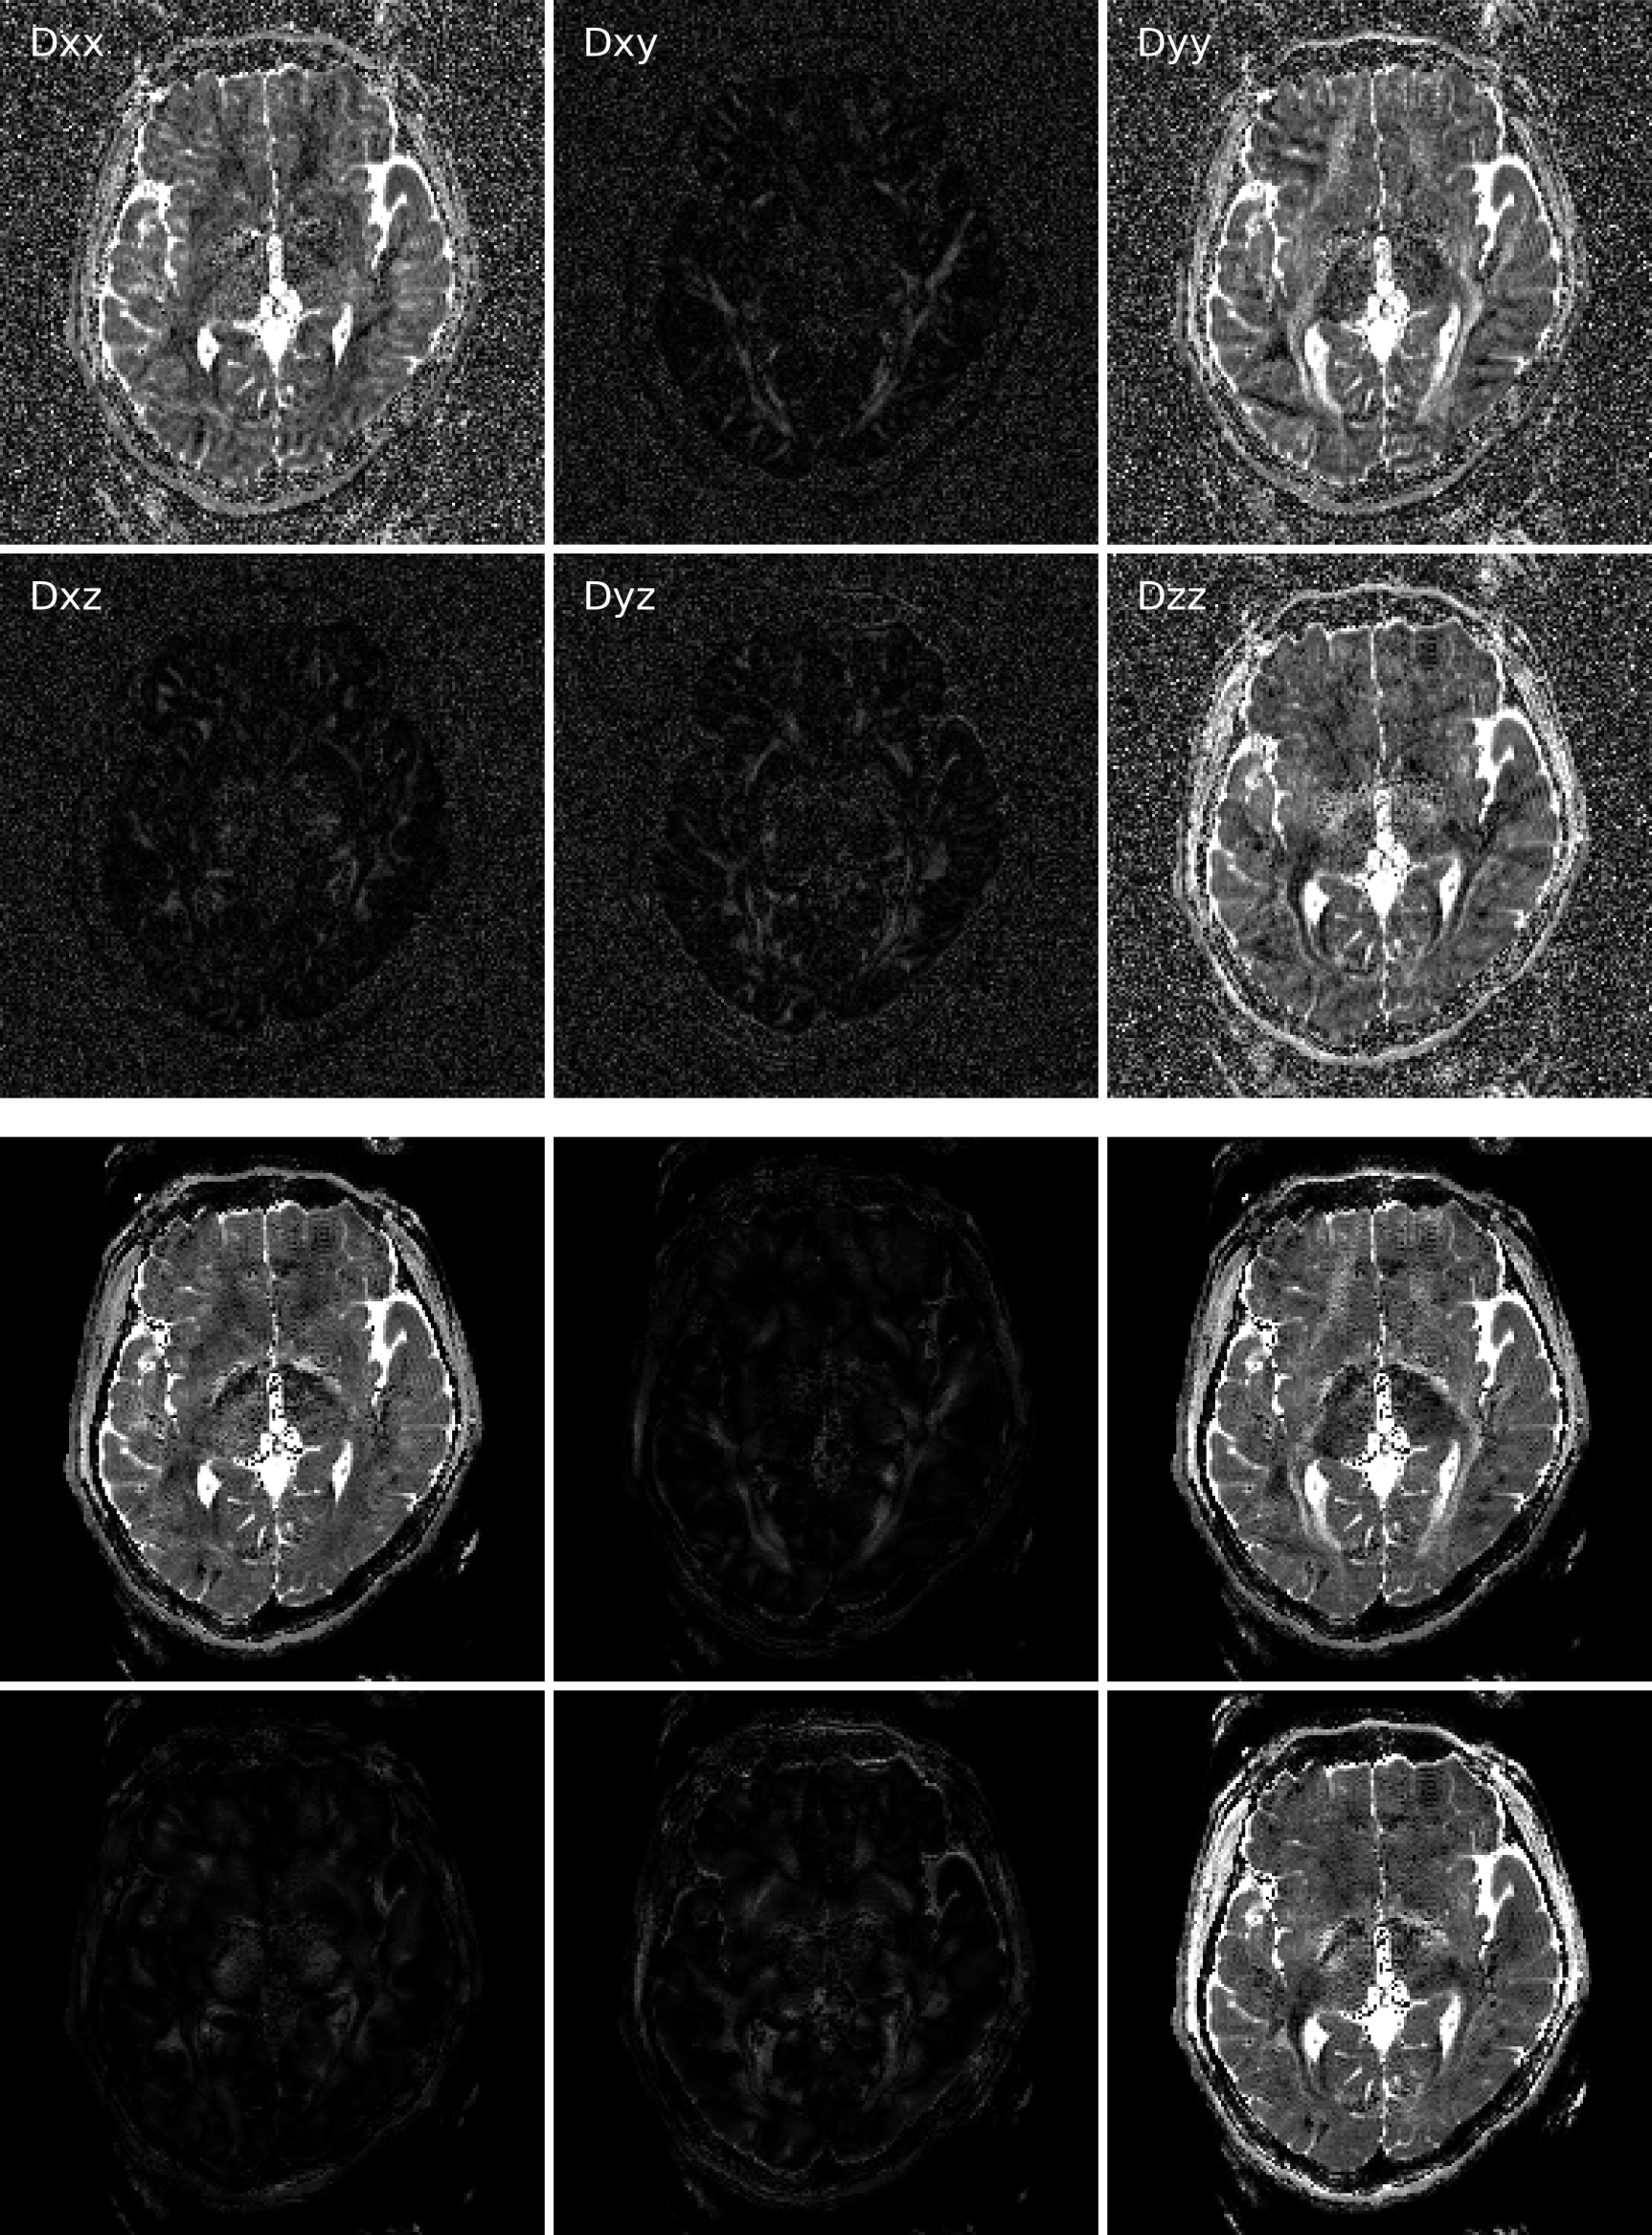
\includegraphics[width=0.4\columnwidth]{dti.png}
				\label{FIG:nlls}
			\end{tikzfigure}
		}
	
		\block{Discussion \& Conclusion}{
			\begin{itemize}
				\item Nonlinear operator abstraction in SigPy;
				\item Nonlinear least square solver with advanced regularization terms;
				\item Examples in \SI{7}{\tesla} diffusion MRI show reasonable results compared to parallel imaging with pixelwise model fitting;
				\item This framework may allow for fast prototyping and testing.
			\end{itemize}
		}
		
		\block{References}{
			\begin{enumerate}
				\item Graff C, et al. Iterative T2 estimation from highly undersampled radial fast spin-echo data. \textit{ISMRM} 2006;14:925.
				\item Block KT, et al. Model-based iterative reconstruction for radial fast spin-echo MRI. \textit{IEEE TMI} 2009;28:1759-1769.
				\item Ong F, et al. SigPy: A Python package for high performance iterative reconstruction. \textit{ISMRM} 2019;27:4819.
				\item Basser PJ, Mattiello J, LeBihan D. MR diffusion tensor spectroscopy and imaging. \textit{Biophys J} 1994;66:259-267.
				\item Breuer F, et al. Controlled aliasing in parallel imaging results in higher acceleration (CAIPIRINHA) for multi-slice imaging. \textit{MRM} 2005;53:684-691.
				\item Boyd S, et al. Distributed optimization and statistical learning via the alternating direction method of multipliers. \textit{Found Trends Mach Learn} 2010;3:1-122.
				\item Cai JF, et al. A singular value thresholding algorithm for matrix completion. \textit{SIAM J Optim} 2010;20:1956-1982.
			\end{enumerate}
		}
%		\note[
%		targetoffsetx=-8cm, 
%		targetoffsety=-11cm, 
%		width=0.4\linewidth
%		]
%		{e-mail: \texttt{zhengguo.tan@fau.de}}
	\end{columns}
	
	
\end{document}
